\begingroup
\newsavebox{\patternfigurebox}
\newsavebox{\planartilefigurebox}
\newsavebox{\woventilefigurebox}
\newcommand{\motivationfigureheight}{0.40\textheight}

\sbox{\patternfigurebox}{%
  \resizebox{!}{\motivationfigureheight}{%
    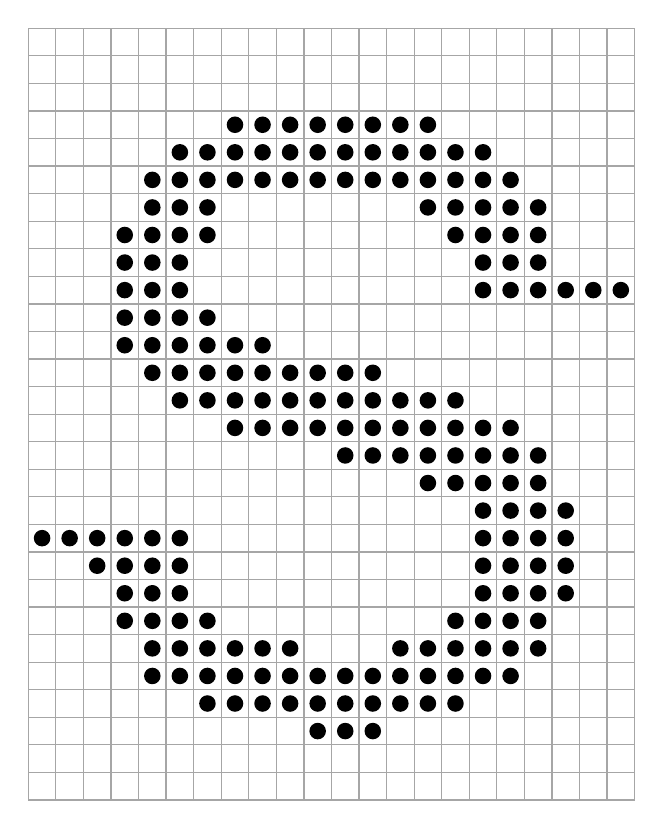
\begin{tikzpicture}[
  x=0.35cm,
  y=0.35cm,
  gridline/.style={
    draw=black!35,
    line width=0.45pt
  },
  patternpoint/.style={
    fill=black,
    draw=none
  }
]

\draw[gridline] (0,0) grid[xstep=1,ystep=1] (22,-28);

\newcommand{\drawpatternrow}[2]{%
  \foreach \tile [count=\c from 0] in {#2} {
    \ifnum\tile=8\relax
    \else
      \fill[patternpoint] ({\c+0.5},{-#1-0.5}) circle[radius=0.3];
    \fi
  }
}

\drawpatternrow{0}{8,8,8,8,8,8,8,8,8,8,8,8,8,8,8,8,8,8,8,8,8,8}
\drawpatternrow{1}{8,8,8,8,8,8,8,8,8,8,8,8,8,8,8,8,8,8,8,8,8,8}
\drawpatternrow{2}{8,8,8,8,8,8,8,8,8,8,8,8,8,8,8,8,8,8,8,8,8,8}
\drawpatternrow{3}{8,8,8,8,8,8,8,2,6,3,2,3,2,6,3,8,8,8,8,8,8,8}
\drawpatternrow{4}{8,8,8,8,8,2,6,7,6,4,5,5,1,3,1,6,3,8,8,8,8,8}
\drawpatternrow{5}{8,8,8,8,2,7,3,1,6,6,4,1,6,4,2,6,7,3,8,8,8,8}
\drawpatternrow{6}{8,8,8,8,1,4,5,8,8,8,8,8,8,8,1,3,1,7,3,8,8,8}
\drawpatternrow{7}{8,8,8,2,3,2,4,8,8,8,8,8,8,8,8,1,3,5,5,8,8,8}
\drawpatternrow{8}{8,8,8,5,5,5,8,8,8,8,8,8,8,8,8,8,5,1,4,8,8,8}
\drawpatternrow{9}{8,8,8,5,5,5,8,8,8,8,8,8,8,8,8,8,1,6,6,6,6,6}
\drawpatternrow{10}{8,8,8,5,1,7,3,8,8,8,8,8,8,8,8,8,8,8,8,8,8,8}
\drawpatternrow{11}{8,8,8,1,3,1,4,2,3,8,8,8,8,8,8,8,8,8,8,8,8,8}
\drawpatternrow{12}{8,8,8,8,1,3,2,4,5,2,6,6,3,8,8,8,8,8,8,8,8,8}
\drawpatternrow{13}{8,8,8,8,8,1,4,2,4,5,2,3,1,3,2,3,8,8,8,8,8,8}
\drawpatternrow{14}{8,8,8,8,8,8,8,1,6,4,1,7,6,7,4,5,2,3,8,8,8,8}
\drawpatternrow{15}{8,8,8,8,8,8,8,8,8,8,8,1,6,4,2,4,5,1,3,8,8,8}
\drawpatternrow{16}{8,8,8,8,8,8,8,8,8,8,8,8,8,8,1,6,7,3,5,8,8,8}
\drawpatternrow{17}{8,8,8,8,8,8,8,8,8,8,8,8,8,8,8,8,1,4,1,3,8,8}
\drawpatternrow{18}{6,6,3,2,6,3,8,8,8,8,8,8,8,8,8,8,2,6,6,4,8,8}
\drawpatternrow{19}{8,8,1,4,2,4,8,8,8,8,8,8,8,8,8,8,1,6,6,3,8,8}
\drawpatternrow{20}{8,8,8,2,7,3,8,8,8,8,8,8,8,8,8,8,2,3,2,4,8,8}
\drawpatternrow{21}{8,8,8,1,4,1,3,8,8,8,8,8,8,8,8,2,4,5,5,8,8,8}
\drawpatternrow{22}{8,8,8,8,2,6,4,2,6,3,8,8,8,2,6,4,2,7,4,8,8,8}
\drawpatternrow{23}{8,8,8,8,1,6,3,1,6,7,3,2,3,1,6,3,1,4,8,8,8,8}
\drawpatternrow{24}{8,8,8,8,8,8,1,6,6,4,5,1,7,6,6,4,8,8,8,8,8,8}
\drawpatternrow{25}{8,8,8,8,8,8,8,8,8,8,1,6,4,8,8,8,8,8,8,8,8,8}
\drawpatternrow{26}{8,8,8,8,8,8,8,8,8,8,8,8,8,8,8,8,8,8,8,8,8,8}
\drawpatternrow{27}{8,8,8,8,8,8,8,8,8,8,8,8,8,8,8,8,8,8,8,8,8,8}

\end{tikzpicture}
%
  }%
}
\sbox{\planartilefigurebox}{%
  \resizebox{!}{\motivationfigureheight}{%
    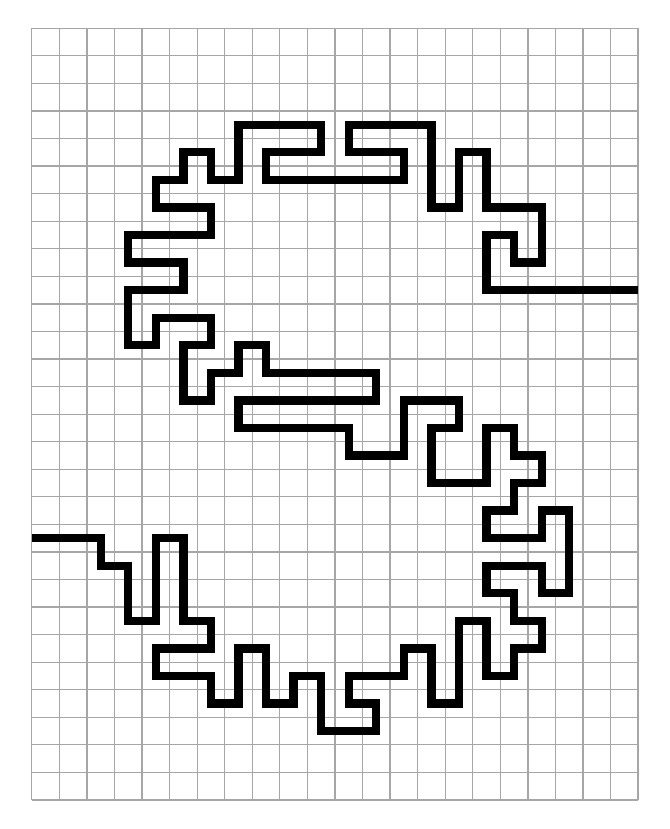
\begin{tikzpicture}[
  x=0.35cm,
  y=0.35cm,
  gridline/.style={
    draw=black!35,
    line width=0.45pt
  },
  pathseg/.style={
    draw=black,
    line width=3pt,
    line cap=butt,
    line join=miter
  }
]

\newcommand{\drawsolutiontile}[1]{%
  \ifcase#1\relax
  \or
    \draw[pathseg] (0.5,0) -- (0.5,-0.5) -- (1,-0.5);
  \or
    \draw[pathseg] (0.5,-1) -- (0.5,-0.5) -- (1,-0.5);
  \or
    \draw[pathseg] (0,-0.5) -- (0.5,-0.5) -- (0.5,-1);
  \or
    \draw[pathseg] (0,-0.5) -- (0.5,-0.5) -- (0.5,0);
  \or
    \draw[pathseg] (0.5,0) -- (0.5,-1);
  \or
    \draw[pathseg] (0,-0.5) -- (1,-0.5);
  \or
    \draw[pathseg] (0.5,0) -- (0.5,-1);
    \draw[pathseg] (0,-0.5) -- (1,-0.5);
  \fi
}

\draw[gridline] (0,0) grid[xstep=1,ystep=1] (22,-28);

\newcommand{\drawsolutionrow}[2]{%
  \foreach \tile [count=\c from 0] in {#2} {
    \begin{scope}[shift={(\c,-#1)}]
      \drawsolutiontile{\tile}
    \end{scope}
  }
}

\drawsolutionrow{0}{8,8,8,8,8,8,8,8,8,8,8,8,8,8,8,8,8,8,8,8,8,8}
\drawsolutionrow{1}{8,8,8,8,8,8,8,8,8,8,8,8,8,8,8,8,8,8,8,8,8,8}
\drawsolutionrow{2}{8,8,8,8,8,8,8,8,8,8,8,8,8,8,8,8,8,8,8,8,8,8}
\drawsolutionrow{3}{8,8,8,8,8,8,8,2,6,6,3,2,6,6,3,8,8,8,8,8,8,8}
\drawsolutionrow{4}{8,8,8,8,8,2,3,5,2,6,4,1,6,3,5,2,3,8,8,8,8,8}
\drawsolutionrow{5}{8,8,8,8,2,4,1,4,1,6,6,6,6,4,5,5,5,8,8,8,8,8}
\drawsolutionrow{6}{8,8,8,8,1,6,3,8,8,8,8,8,8,8,1,4,1,6,3,8,8,8}
\drawsolutionrow{7}{8,8,8,2,6,6,4,8,8,8,8,8,8,8,8,8,2,3,5,8,8,8}
\drawsolutionrow{8}{8,8,8,1,6,3,8,8,8,8,8,8,8,8,8,8,5,1,4,8,8,8}
\drawsolutionrow{9}{8,8,8,2,6,4,8,8,8,8,8,8,8,8,8,8,1,6,6,6,6,6}
\drawsolutionrow{10}{8,8,8,5,2,6,3,8,8,8,8,8,8,8,8,8,8,8,8,8,8,8}
\drawsolutionrow{11}{8,8,8,1,4,2,4,2,3,8,8,8,8,8,8,8,8,8,8,8,8,8}
\drawsolutionrow{12}{8,8,8,8,8,5,2,4,1,6,6,6,3,8,8,8,8,8,8,8,8,8}
\drawsolutionrow{13}{8,8,8,8,8,1,4,2,6,6,6,6,4,2,6,3,8,8,8,8,8,8}
\drawsolutionrow{14}{8,8,8,8,8,8,8,1,6,6,6,3,8,5,2,4,2,3,8,8,8,8}
\drawsolutionrow{15}{8,8,8,8,8,8,8,8,8,8,8,1,6,4,5,8,5,1,3,8,8,8}
\drawsolutionrow{16}{8,8,8,8,8,8,8,8,8,8,8,8,8,8,1,6,4,2,4,8,8,8}
\drawsolutionrow{17}{8,8,8,8,8,8,8,8,8,8,8,8,8,8,8,8,2,4,2,3,8,8}
\drawsolutionrow{18}{6,6,3,8,2,3,8,8,8,8,8,8,8,8,8,8,1,6,4,5,8,8}
\drawsolutionrow{19}{8,8,1,3,5,5,8,8,8,8,8,8,8,8,8,8,2,6,3,5,8,8}
\drawsolutionrow{20}{8,8,8,5,5,5,8,8,8,8,8,8,8,8,8,8,1,3,1,4,8,8}
\drawsolutionrow{21}{8,8,8,1,4,1,3,8,8,8,8,8,8,8,8,2,3,1,3,8,8,8}
\drawsolutionrow{22}{8,8,8,8,2,6,4,2,3,8,8,8,8,2,3,5,5,2,4,8,8,8}
\drawsolutionrow{23}{8,8,8,8,1,6,3,5,5,2,3,2,6,4,5,5,1,4,8,8,8,8}
\drawsolutionrow{24}{8,8,8,8,8,8,1,4,1,4,5,1,3,8,1,4,8,8,8,8,8,8}
\drawsolutionrow{25}{8,8,8,8,8,8,8,8,8,8,1,6,4,8,8,8,8,8,8,8,8,8}
\drawsolutionrow{26}{8,8,8,8,8,8,8,8,8,8,8,8,8,8,8,8,8,8,8,8,8,8}
\drawsolutionrow{27}{8,8,8,8,8,8,8,8,8,8,8,8,8,8,8,8,8,8,8,8,8,8}

\end{tikzpicture}
%
  }%
}
\sbox{\woventilefigurebox}{%
  \resizebox{!}{\motivationfigureheight}{%
    \input{figures/s-sol-grid.tex}%
  }%
}

\begin{tikzpicture}[
  graphic/.style={
    inner sep=0pt,
    outer sep=0pt
  },
  flow/.style={
    -{Stealth[length=2.5mm,width=1.8mm]},
    draw=black,
    line width=1.1pt,
    shorten <=2pt,
    shorten >=2pt
  }
]
  \node[graphic] (planar-tiles) {\usebox{\planartilefigurebox}};
  \node[graphic, below=0.42cm of planar-tiles]
    (woven-tiles) {\usebox{\woventilefigurebox}};

  \node[graphic, right=0.85cm of planar-tiles]
    (planar-maze) {%
      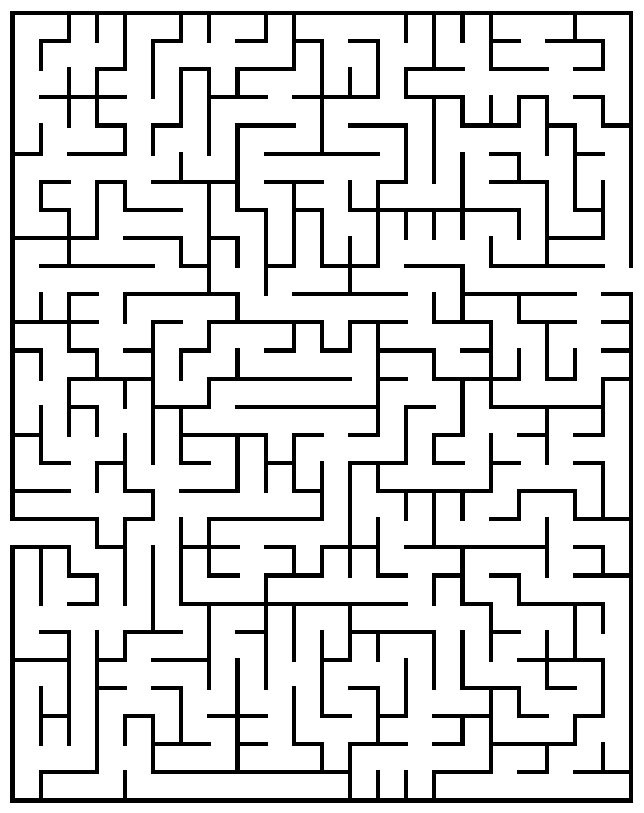
\includegraphics[height=\motivationfigureheight]{figures/s-no-solution.pdf}%
    };
  \node[graphic, right=0.85cm of woven-tiles]
    (woven-maze) {%
      
\includegraphics[height=\motivationfigureheight]{figures/crossed-s-no-solution.pdf}%
    };

  \node[graphic, right=0.85cm of planar-maze]
    (planar-solution) {%
      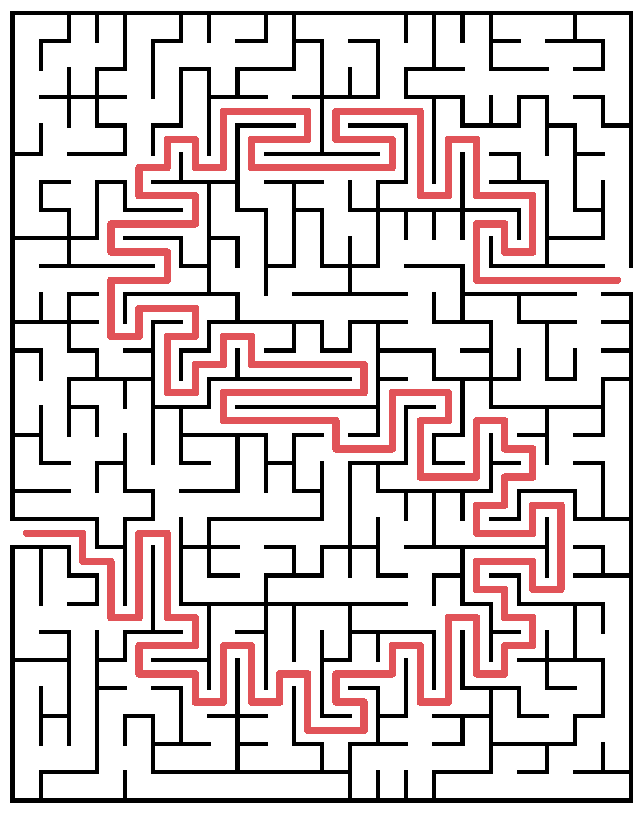
\includegraphics[height=\motivationfigureheight]{figures/s.pdf}%
    };
  \node[graphic, right=0.85cm of woven-maze]
    (woven-solution) {%
      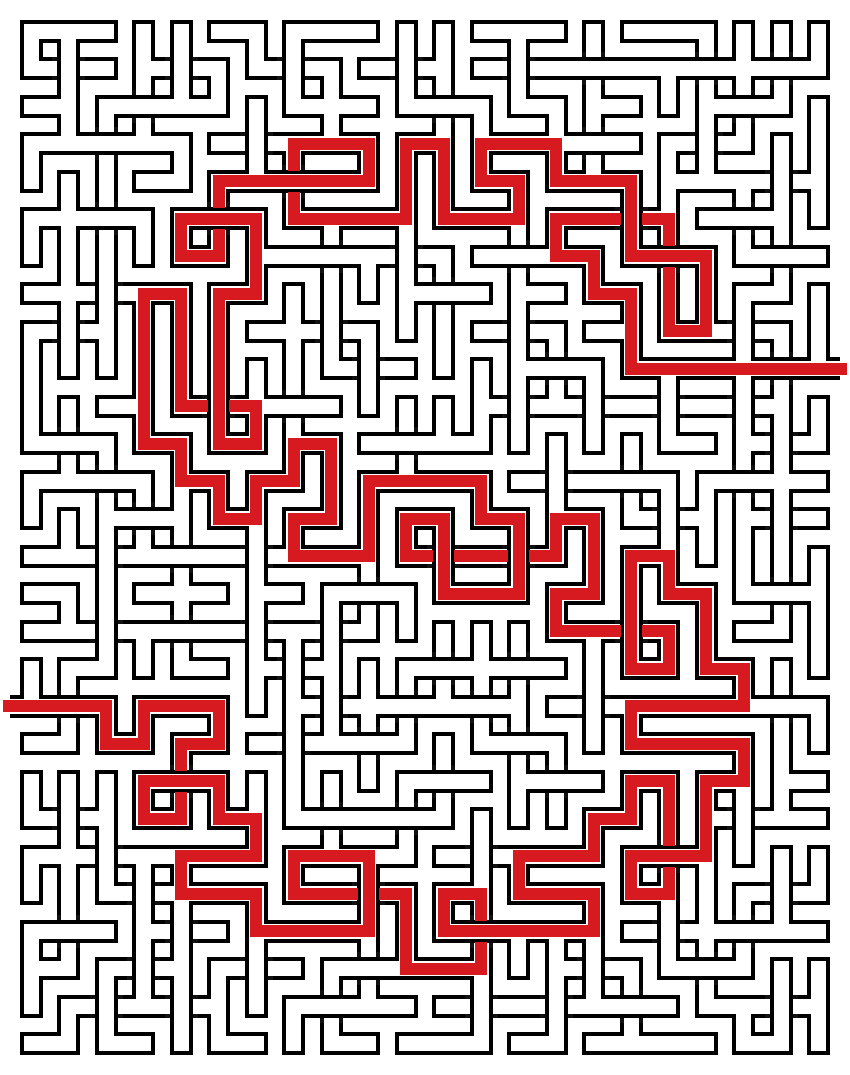
\includegraphics[height=\motivationfigureheight]{figures/crossed-s.pdf}%
    };

  \coordinate (branch-center) at
    ($(planar-tiles.west)!0.5!(woven-tiles.west)$);
  \node[graphic, left=1.05cm of branch-center]
    (pattern) {\usebox{\patternfigurebox}};

  \draw[flow] (pattern.east) to[out=24,in=180] (planar-tiles.west);
  \draw[flow] (pattern.east) to[out=-24,in=180] (woven-tiles.west);
  \draw[flow] (planar-tiles.east) -- (planar-maze.west);
  \draw[flow] (planar-maze.east) -- (planar-solution.west);
  \draw[flow] (woven-tiles.east) -- (woven-maze.west);
  \draw[flow] (woven-maze.east) -- (woven-solution.west);
\end{tikzpicture}
\endgroup
